\glsresetall

\section{CUDSwap: Tolerating Memory exhaustion failures in cloud computing}\label{section_cudswap}

Cloud computing is now being used by a wide variety of users, ranging from
expert programmers and system administrators to scientists and laymen.
Cloud providers are taking full advantage of all their resources as much as
they can. Memory is the most expensive resource in terms of oversubscription
and this has resulted in high price to the end user. Furthermore, performing
swapping in \gls{vm} is expensive, so the cloud providers
usually do not offer any swapping space for their systems. As a consequence,
when a \gls{vm} runs out of memory, user processes are killed. This scenario in
cloud environment is especially critical, since the user loses all of
his/her execution time and, by extension, the money invested in this
computation. For cloud users such as life scientists with varying memory
requirements, this is a critical problem. This paper presents CUDSwap,
a kernel extension module designed to detect memory exhaustion in cloud
instances, add more swap space, and thus prevent process failures. CUDSwap
has been implemented in Linux kernel and has been evaluated over a variety
of workloads as well as real-world life science applications. The paper
describes CUDSwap design and implementation details, and reports performance
details from the evaluation.

\subsection{Introduction}\label{sub_cudswap_Introduction}

Cloud computing is being used in a wide variety of fields, including web
hosting, media content, scientific computing, and many more. This wide range
implies that the cloud users are not necessarily computing experts,
especially in the world of scientific computing that includes biologists,
physicists, chemists, etc. From our past experience working with scientists,
we have found that their experience with the cloud is often quite poor,
and sometimes they feel that they are wasting money using the cloud. Usually,
scientists do not have an a priori idea of the amount of various computing
resources they will need to complete their computing tasks. Typically,
they perform a rough estimation of the resources they will need and launch
the cloud instance that they think will be enough to run their applications.
An incorrect estimation of required resources can lead to poor performance
and even complete failure. In the case of an incorrect CPU estimation, the
application will simply take longer to finish, but the work is not lost.
In the case of incorrect storage estimation, the user can dynamically add
more storage to the instance, so that the application can continue working
without any problem.

However, the most critical resource is memory, because when it is exhausted,
the application is aborted and all the work done by the application is lost.
This is because cloud providers usually don't provide any swap space in
their instances due to high impact on the performance of
their systems. As a result, when a user's virtual machine (VM) doesn't have
enough memory to execute all the running applications, user processes are
killed in order to keep the VM alive. In Linux systems, processes are
killed using the Out Of Memory Killer (OOM Killer), a kernel module that
prevents the Out Of Memory machine state in the VM. This memory exhaustion
failure not only results in poor user experience, but also results in a large
financial loss for the user. All the work done before a process is killed is
lost and all the money invested in these processes
is wasted. Furthermore, the user has to start a new, larger VM, increasing
the total cost for the user.

In this paper, we address this memory exhaustion failure problem in VM
instances by introducing CUDSwap, an elegant kernel module that requires
minimal changes to the current Linux kernel. This module is designed to
avoid the OOM Killer calls by increasing the amount of virtual memory on
the fly. CUDSwap is a dynamic kernel module that monitors the amount of
free system memory, and adds swap space whenever needed, so that the
application process is not killed. We have implemented a prototype of
CUDSwap for Linux kernel and evaluated it extensively for a variety of
applications ranging from artificial workloads to real-world, life science
applications on Amazon EC2. This evaluation demonstrates that CUDSwap
prevents memory exhaustion failures of applications running on cloud. In
addition, CUDSwap improves user experience and even reduces the total
cost of running applications on cloud. We provide a detailed cost benefit
analysis of using CUDSwap.

By using a dynamic approach, CUDSwap uses the storage space only when it
is strictly needed. Furthermore, with increasing use of cloud in areas
beyond computer science, a large number of users do not have enough
computing background to create swap space before running their program.
CUDSwap creates swap space for them. Another advantage of CUDSwap is in
the case where a user is unable to accurately predict her program memory
requirement. In some applications, it is hard to predict the amount of
memory they will need and the user may make an incorrect approximation
that may result in provisioning insufficient memory to its processes.
CUDSwap enables such processes to complete their execution.

The remainder of this paper is organized as follows. Section \ref{sub_cudswap_Work}
provides a brief review of some important related work. Section \ref{sub_cudswap_VMs}
describes the details of how VMs manage memory exhaustion at present.
Section \ref{sub_cudswap_Design} describes the design approach of the system.
Section \ref{sub_cudswap_Implementation} describes the Linux implementation details of
CUDSwap. Section \ref{sub_cudswap_Evaluation} discusses the performance results, as well
as a cost benefit analysis. Finally, Section \ref{sub_cudswap_Conclusion} discusses
future directions and concludes the paper.

\subsection{Related Work}\label{sub_cudswap_Work}

Earlier work on memory exhaustion failures in the cloud has not been
focused on the users point of view. They are targeted to provide solutions
to the memory oversubscription problem from the provider's point of view,
i.e. the impact on the physical machine as a result of running several VMs
on it. There are mainly two approaches to this problem: VM migration and
Network Memory.

Systems that provide VM migration are Xen \cite{Barham2003},
VMWare's VMotion \cite{Nelson2005} and SnowFlock \cite{Lagar-Cavilla2009},
among others. These systems move a VM that is hosted in a machine with not
enough memory and re-deploys it in a new machine. They provide support for
reconfiguring a VM in a new physical machine with enough resources to
fulfill VM's requirements. They are tailored to support sustained periods of
memory oversubscription. The main disadvantage of this approach is the VM
downtime. In order to be able to migrate the VM from one physical machine
to another, it has to be suspended in the old machine and resumed in the
new one. Although live migration techniques allow VM migration with minimal
downtime, they still have to face the problem of network link saturation.

Systems using the Network Memory approach include Cellular Disco
\cite{Govil2000}, Cooperative Caching \cite{Dahlin1994} and Nswap
\cite{Newhall2003}, among others. These systems are designed to
support short memory overloads. They create a new level on memory hierarchy by
adding a new level of memory cache between the main memory and the disk,
located across the network. A large number of these systems use the concept
of cooperative memory, which consists of performing memory swapping across
the network. The swapped out pages are stored in remote page repositories.
Earlier research has shown that cooperative memory has better performance
that disk swap \cite{Anderson1995}. However, these systems do not support
long periods of memory oversubscription and are tailored for short bursts
of memory overloads. The performance of these
systems degrades significantly when the duration of the overload increases
due to network bottleneck.

Recently, hybrid systems have been proposed in order to take advantage of
the VM migration and Network Memory benefits. One such system is Overdriver
\cite{Williams2011}, which monitors the memory overload and creates
adaptive thresholds. Based on these thresholds, the system decides between
performing Cooperative Swap or VM migration.

However, all the above-described systems do not solve the problem of the
memory exhaustion on the client VM instance. CUDSwap differs from these
earlier approaches from the memory overload point of view. While earlier
approaches tried to overcome the challenge of memory exhaustion failure by
managing the physical memory of the host machine, we address the problem
from the guest VM's point of view. This way, we are giving the opportunity
to the end user to choose between different VM configurations knowing that
her applications will be completed and she can decide based on
performance-cost tradeoffs. In \cite{Molina2013dcdv},
we provided an analysis of this problem and proposed a preliminary
solution for it. However, that solution relies on a heuristic that can
potentially miss an Out Of Memory state, resulting in the OOM Killer being
called. The heuristic is based on the default memory threshold (3\% of the
total memory) that Linux  uses to kill a process if the system is hitting
the OOM state. Specifically, CUDSwap uses a 7\% threshold, which is checked
at the time a process requests more memory. However, it does not take into
account the amount of memory requested by the process, so if it requests
more than $7\% - 3\% = 4\%$ of the total amount of memory, CUDSwap will
miss the OOM state and the process will be killed. Here, we will describe
the improvements we have made in the design and implementation of CUDSwap
based on our experience in \cite{Molina2013dcdv}.

\subsection{Memory Exhaustion in VMs}\label{sub_cudswap_VMs}
The Out Of Memory (OOM) machine state is an undesired state where the
kernel is not able to allocate more memory because there isn't sufficient
virtual memory available, i.e. the main memory space and the swap space
(in case of its existence) are full. In this scenario, the Linux kernel
tries to free up memory using the OOM Killer \footnote{\url{http://linux-mm.org/OOM_Killer}}.
The OOM Killer is a kernel system tailored to free up memory by killing processes.

The OOM Killer is the last resource used by the kernel to free up memory,
since the kernel always tries to keep all the user processes alive.
Killing processes is a critical operation, so the OOM Killer has to decide
which process is the most appropriate to be killed. The OOM Killer is
designed in a way that it tries to free up as much memory as possible by
killing as few processes as possible (only one if it is possible), and
lose as little work done (by killed processes) as possible. In order to do
so, the OOM Killer assigns a {\it rank} for each process following a set
of rules. The rank for each process is computed in a cumulative manner.
Each process is continuously assigned points and the process that has
more points is more likely to be a candidate for termination. The process
rank is initialized with the amount of resident memory allocated by the
process. The independent allocated memory of each child process (excluding
kernel threads) is then added to the parent rank. After this, the process
rank is decreased regularly by the CPU and run times. This way, processes
running for a long time are more likely to be kept alive, fulfilling the
premise of losing the minimum amount of work done.

The rank of {\it niced}  processes is doubled because they are likely less
important. Next, processes with the {\it CAP\_SYS\_ADMIN} or
{\it CAP\_SYS\_RAWIO} capabilities have their ranks reduced, since these
processes have rights to perform system administration operations and
input/output operations, respectively. They may leave the system in an
inconsistent state if killed. Finally, the process rank is shifted by the
value in {\it /proc/$<$pid$>$/oom\_adj}, which is a user-defined value
and set to its parent value by default.

The final result of following this procedure to determine which process
to kill when needed is that the processes that are killed are less
important (niced), use lots of memory, have not so far executed for long,
and are not performing any input/output operations.

\subsubsection{OOM Checklist}

Before calling the OOM Killer, the out of memory manager should go through a checklist in order to ensure that the OOM Killer is called if and only if it is necessary. This checklist performs the following steps:

\begin{enumerate}
\item Is there enough swap space left? If yes, do not call OOM.
\item Has it been more than five seconds since last failure? If yes, do not call OOM.
\item Have we failed within the last second? If no, do not call OOM.
\item Has it been ten failures at least in the last five seconds? If no, do not call OOM.
\item Has a process been killed within the last five seconds? If yes, do not call OOM.
\end{enumerate}

This checklist ensures that the system is really out of memory and it is not, for example, waiting for I/O to complete for pages swapped to disk.

\subsection{CUDSwap Design}\label{sub_cudswap_Design}

In order to prevent calls to the OOM killer, CUDSwap needs to perform three
important functions. First, it needs to monitor the available free space
in memory. Second, it needs to suspend a process requesting new memory
whenever the available free space goes below some threshold and create
additional swap space. Finally, it needs to wake the suspended process after
additional swap space has been created. CUDSwap consists of
two main modules: {\it mod\_hack\_brk} and {\it swap\_creator} (See
Figure \ref{cudswapfigure1}).

\begin{figure}[htbp]
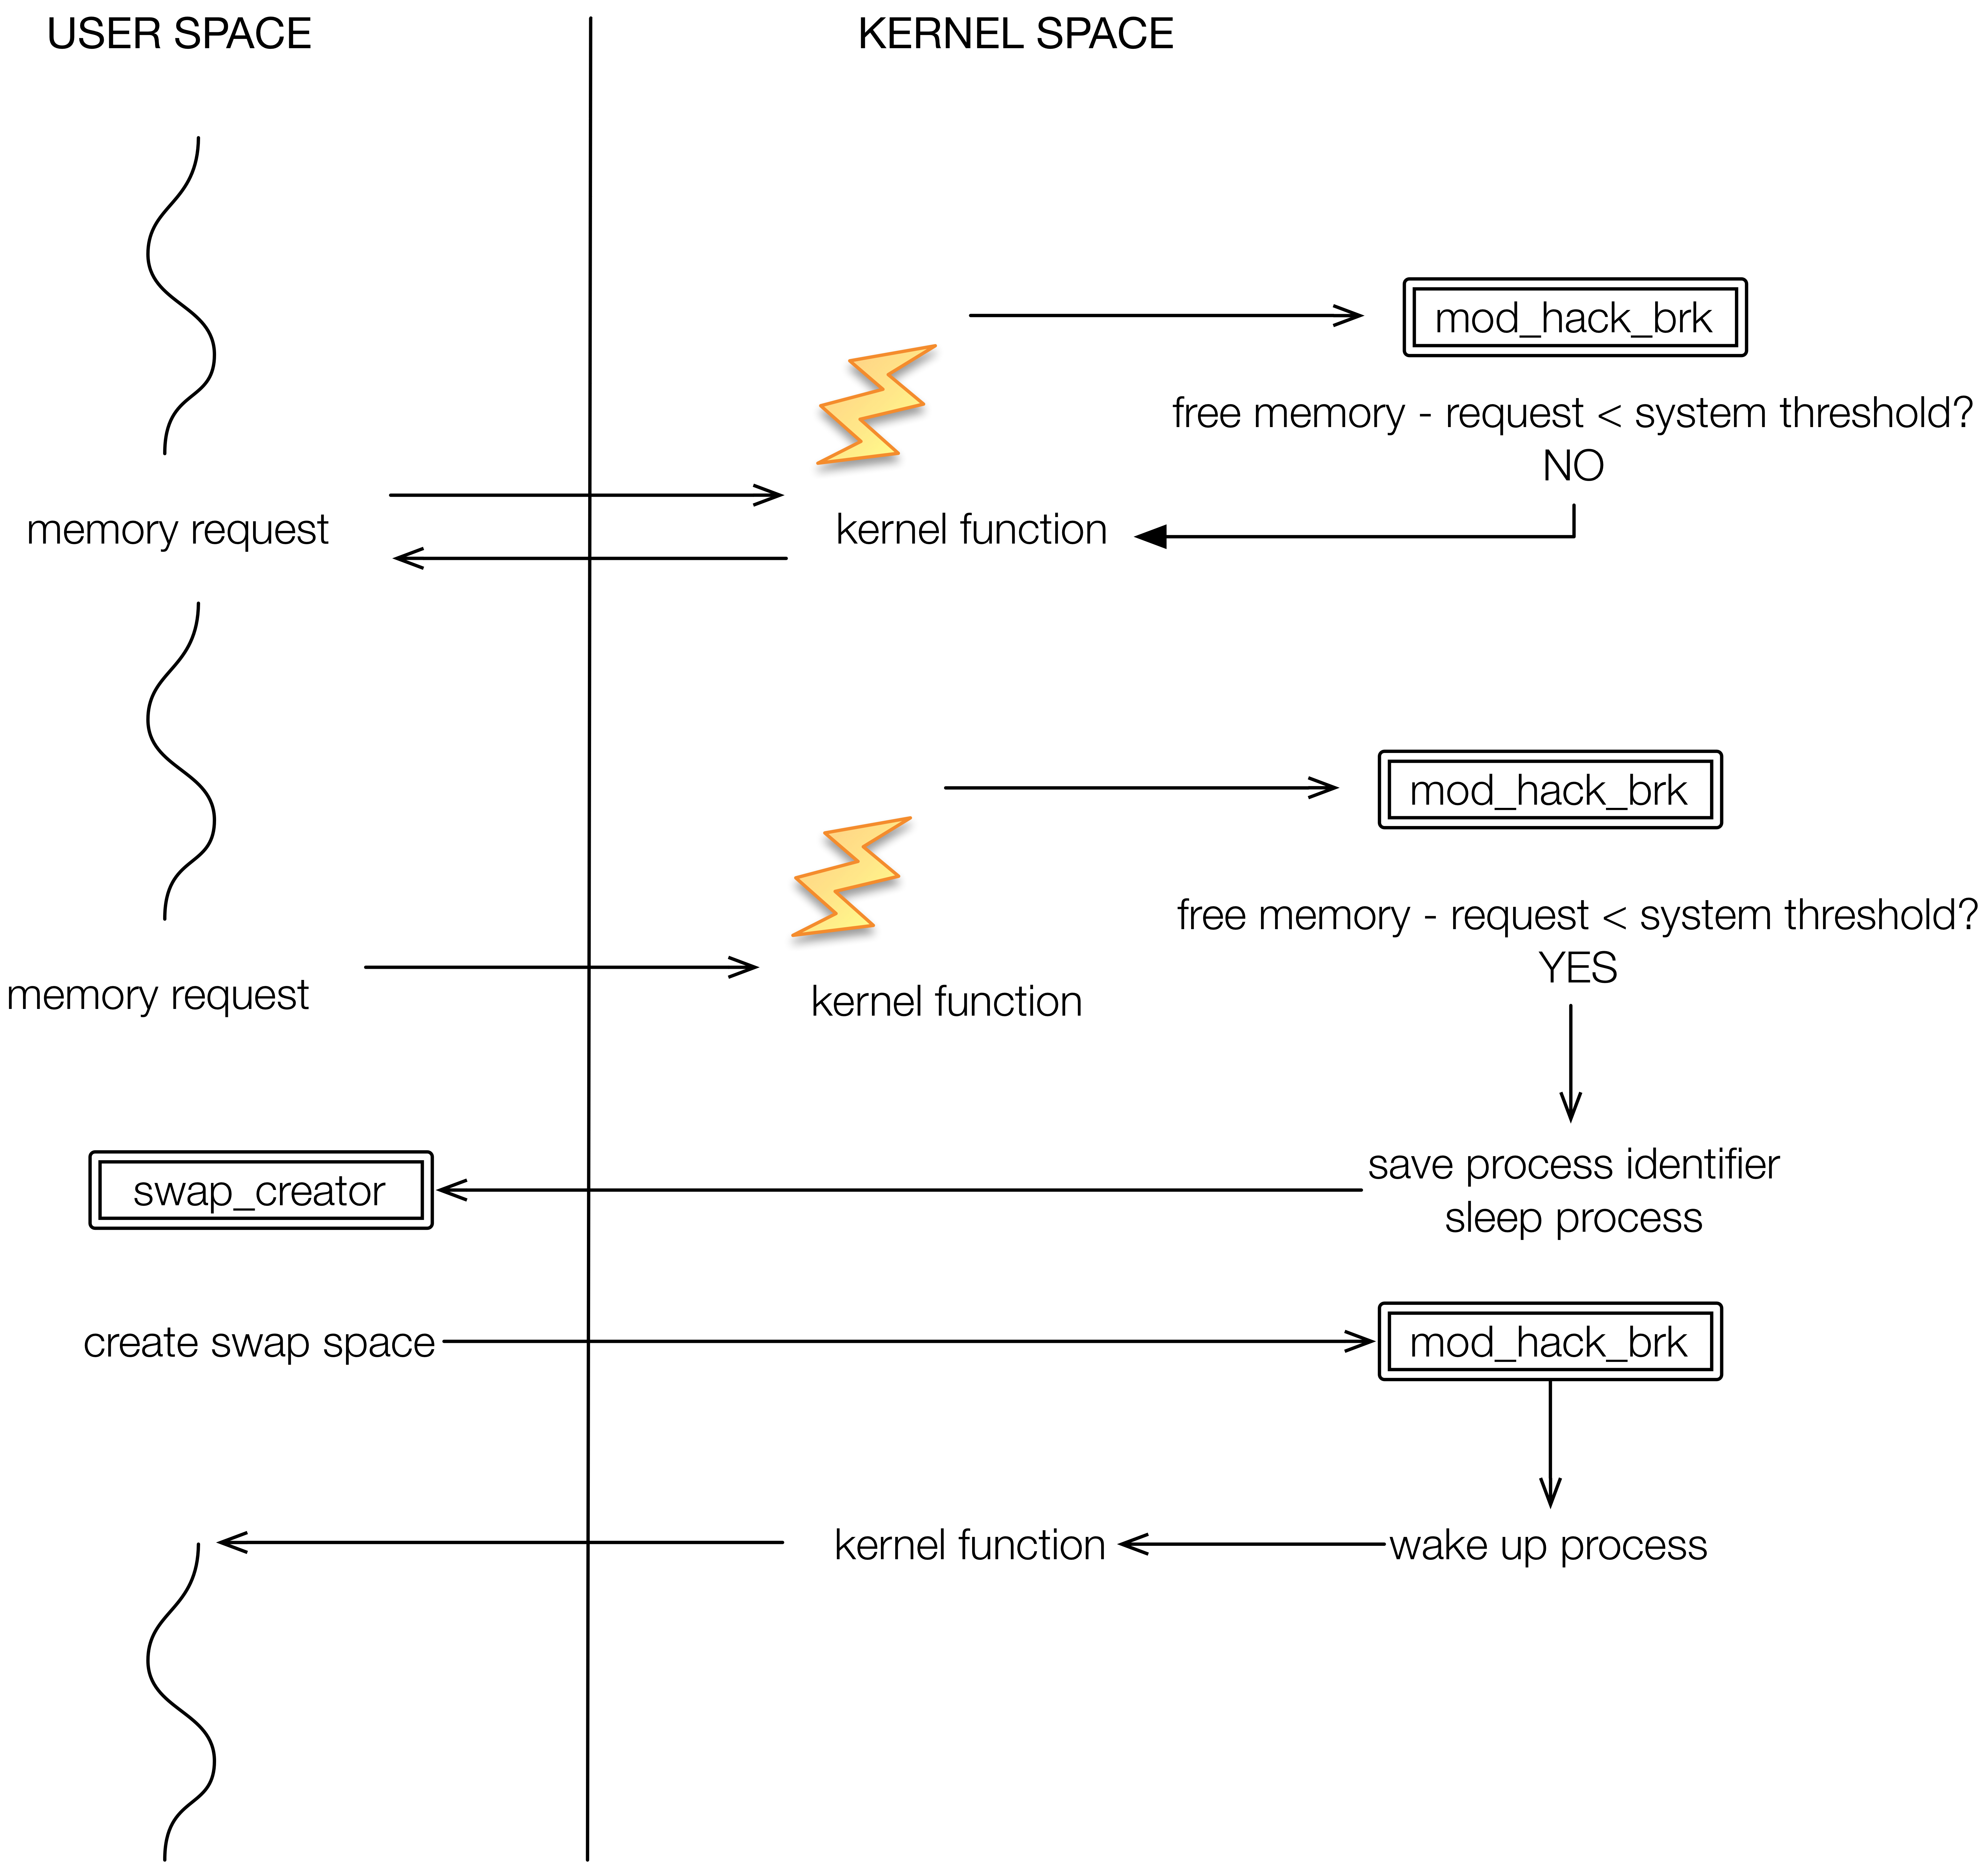
\includegraphics[width=\columnwidth]{chapter_cudswap_figures/Figure_1.jpg}
\caption[Design Overview]{\textbf{Design Overview.}}
\label{cudswapfigure1}
\end{figure}

\subsubsection{mod\_hack\_brk Module}

The {\it mod\_hack\_brk} module is tailored to monitor the free memory
of the system and suspend the current process if its current memory request
will produce a memory exhaustion failure.. By default, the Linux kernel sets a threshold in order to know if the machine is in the out of memory state. This
threshold is placed at 3\% of the total amount of virtual memory present
in the system. This way, the kernel has enough memory to run the OOM Killer,
if needed. The {\it mod\_hack\_brk} module essentially checks if the free
memory will go below this threshold if more memory is allocated to a process.

A key question is when should the {\it mod\_hack\_brk} module check whether
the amount of free memory has fallen below the threshold at 3\% of the
total amount of system's virtual memory. There are two options:
perform a periodic poll or check each time a process
requests more memory. The former has the problem that it will introduce an
overhead in the system even if the system is idle. Another important
drawback of this solution is that we have to manage a trade-off between
the polling time period and the overhead introduced due to polling: if the
polls are not sufficiently frequent, we may miss an out of memory state,
which may result in a process being killed. On the other hand, if the polls
are too frequent, the introduced polling overhead will be prohibitive.

For these reasons, we decided to check the amount of free memory each time
a process requests more memory.
Each time a process requests more memory from the kernel, the
{\it mod\_hack\_brk} module intercepts the requests and checks if the
amount of free memory in the system minus the amount of memory requested
by the process is below the system threshold. If so, it puts the requester
process to sleep, saves the process id of that process, and then
wakes up the {\it swap\_creator} module (described below) to create new
swap space. After new swap space has been created, the {\it swap\_creator}
process notifies the {\it mod\_hack\_brk} module, which wakes up all the
processes that were put to sleep. This solution ensures that only processes
that have requested more memory than available in the system are put in
sleep mode, while memory requests of processes requesting smaller amounts
of memory are satisfied.

There are two main system calls that can be used by a process to modify its
data segment: {\it do\_mmap} and {\it do\_brk}.
The {\it mod\_hack\_brk} module intercepts these system calls and, before they
are executed, checks the available memory in the system. The main drawback
of this solution is that it introduces an overhead each time the
{\it do\_brk} or {\it do\_mmap} system call is executed, but it avoids the
trade-off described above regarding the polling solution.

\subsubsection{swap\_creator Module}

The {\it swap\_creator} module is a process that runs with root privileges
in user space and its main function is to create new swap space whenever
needed. During most of its lifetime, this process is sleeping and it is
woken up by the {\it mod\_hack\_brk} module only when new swap space is
needed.

Once this process is woken up, it performs three important steps. First,
it creates a 2GB file with no holes (i.e. it is not a sparse file and it
is zeroed). Second, it creates a child process that executes the
{\it mkswap} command on the created file. Finally, the {\it swap\_creator}
process mounts the created file as a swap space, increasing the amount of
virtual memory. After this final step, this process notifies the
{\it mod\_hack\_brk} module, and goes back to sleep.

\subsubsection{Design Discussion}

The functionality of creating new swap space is implemented as a
separate module ({\it swap\_creator} module) running in the user space.
The main reason why this functionality is not integrated within the
{\it mod\_hack\_brk} module is that it is a bad idea in general to open
files from the kernel space. I/O operations are the source of a large
number of errors, and one of these errors in the kernel space will cause
the entire system to crash. Hence, having these operations in user space
makes CUDSwap more robust.

We highlight the fact that in this design, new swap space is created
strictly if it is needed, i.e. if the amount of free memory in the system
minus the amount of memory requested by the process is below the system
threshold. This is different from our earlier design \cite{Molina2013dcdv}
where new swap space was created if there was a likelihood of memory
exhaustion. After performing several experiments, we concluded that
this higher threshold is too conservative. We observed that it
resulted in wasting system resources most of the time, i.e. new swap
space was created when the available free memory would not have fallen
below 3\% and hence OOM Killer process wouldn't have been invoked.

In addition, the system design has been simplified from our earlier
design. The {\it wake\_up} module from the earlier implementation has been
removed and its functionality has been included in the {\it mod\_hack\_brk}
module. The main reason for this change was to improve security
and reliability of the system. The process identifiers are no longer
stored in a configuration file, they are stored in memory in the
{\it mod\_hack\_brk} module. This way, the process identifiers are no
longer exposed to the file system, which can be targeted by third party
applications that can modify it, adding or removing process ids, resulting
in an undesired behavior in the system. This change also simplifies the
functionality of the {\it swap\_creator} module. It no longer needs to
manage the process ids of the processes that need to be woken up.

\subsection{CUDSwap Implementation}\label{sub_cudswap_Implementation}

\subsubsection{Intercepting do\_brk and do\_mmap}

We need to not only intercept {\it do\_brk} or {\it do\_mmap} calls,
but also have access to the amount of memory that the process is requesting.
This information can be obtained using Jprobes \cite{Mavinakayahalli1006Linux}, another
flavor of Kprobes \cite{Krishnakumar2005} that gives access to the function call
parameters. Jprobes is a kernel debugger system that allows the module
programmers to add functions before and after a certain system call is
executed. This way, we can introduce a function before the {\it do\_brk}
system call is executed, and the {\it mod\_hack\_brk} module can perform
the needed checks to ensure the minimum free virtual memory to avoid
the OOM Killer calls. Using the parameters of the system call, we can
compute the amount of memory that the process is requesting, so we can
deterministically decide whether the system has enough memory to handle
the request.

\subsubsection{Getting Memory Information}

We obtain memory information directly from kernel routines. The Linux
kernel provides two different routines for getting the memory information:
{\it si\_meminfo} and {\it si\_swapinfo}. The former provides the
information of the RAM usage, while the latter provides the information of
the swap space. However, the {\it si\_swapinfo} routine is not exported to
the Loadable Kernel Module (LKM) space. We address this problem by
recognizing that the two routines have the same signature and their usage
in the LKM does not incur any security issue. Thus, we have modified the
Linux kernel source to export the {\it si\_swapinfo} routine and then use
it in our {\it mod\_hack\_brk} module. We should highlight that this is the
the only change needed in the current Linux kernel.

This process of obtaining memory information directly from the kernel
routines is a significant change from our earlier implementation that read
memory information from the {\it /proc/meminfo} file. This change completely
removes the interaction of the kernel with the file system, removing any
source of kernel failure due to this interaction.

\subsubsection{mod\_hack\_brk - swap\_creator Communication}

The {\it mod\_hack\_brk} and {\it swap\_creator} modules have to communicate
in both directions. The {\it mod\_hack\_brk} module needs to wake up
the {\it swap\_creator} module whenever new swap space is needed, and the
{\it swap\_creator} module needs to communicate with the
{\it mod\_hack\_brk} module after the new swap space has been created.
The former communication is challenging because we have to perform
communication from the kernel space to the user space. Furthermore, the
{\it swap\_creator} process is a root process and the active process during
the execution of {\it mod\_hack\_brk} may be a non-root process without
privileges to send a signal to a root process. However, both problems are
solved because we have access to the signal primitives. Using the signal
primitives, we can provide the entire {\it task\_struct} of the receiving
process, and our signals do not go through the privilege checks.

For communication from the {\it swap\_creator} process to the
{\it mod\_hack\_brk} module, the {\it mod\_hack\_brk} module creates a
new entry on the /proc virtual file system and the {\it swap\_creator} process only
writes a single value to notify that the swap space has been successfully
created. This implementation is much more secure than our earlier
implementation, since the process ids are no longer provided through the
/proc file system and the {\it mod\_hack\_brk} module can ensure that the
process ids that it has are correct and secure to use.

\subsection{CUDSwap Evaluation}\label{sub_cudswap_Evaluation}

To evaluate the performance of CUDSwap, we have used four different workloads:
\begin{enumerate}
\item Workload 1: An artificial application that executes ten times a large
chunk of memory allocation and performs a sequential write followed by a
sequential read on it.

\item Workload 2: An artificial application that allocates a large chunk of
memory and performs a random write followed by a random read on the entire
chunk of memory.

\item Workload 3: An artificial application that executes Workload 1, and
in parallel also executes a process that continuously writes a large file
to disk, in order to stress the I/O system.

\item Workload 4: A real-world, bioinformatics application. We have used
the sequence clustering step on the QIIME pipeline \cite{Caporaso2010}
using the
UCLUST algorithm \cite{Edgar2010}. This step takes a sequence file with the
input sequence and a reference file with the cluster sequence seeds. It
then parses the input file and tries to group the input sequence with
reference seeds such that they are similar above some user-defined threshold.
\end{enumerate}

In order to conduct our experiments, we have used three different instances
of Amazon EC2 \footnote{\url{http://www.amazon.com/ec2}}: Micro, Small and Medium instances. Table
\ref{cudswaptable1} shows the characteristics of these instances. We decided
to use a real cloud to conduct our experiments in order to remove the potential
infrastructure differences present in a controlled lab environment. Instead,
our controlled set of applications that exhibits different memory behaviors
(including a real-world scientific application) provides much more realistic
performance measures.

\begin{table}[htbp]
\centering
\caption[Selected instance configurations]{Selected instance configurations.}\label{cudswaptable1}
\begin{tabular*}{\textwidth}{ccccc}
\toprule
Instance & CPU & Memory & Storage & Price\\
\midrule
Micro & 1 or 2 ECU & 615 MB & EBS only & \$0.02 per hr\\
\midrule
Small & 1 ECU & 1.7 GB & 160 GB & \$0.06 per hr\\
\midrule
Medium & 2 ECU & 3.75 GB & 410 GB & \$0.12 per hr\\
\bottomrule
\end{tabular*}
\end{table}

\subsubsection{Micro vs Small Instance}
\label{micro-small}

In our first experiment, we compare the performance of running the four
workloads on Micro instance versus running them on Small
instance. For the Workloads 1, 2 and 3, we have used 1 GB of memory, which
is considerably larger than the amount of memory available on the Micro
instance. For the Workload 4, we have used a subset of 1,000,000 input
sequences from Yatsunenko human gut microbiome study \cite{Yatsunenko2012} and the
94\% representative sequence set from the GreenGenes database \cite{DeSantis2006}.
With these parameters, Workload 4 uses about 0.7 GB of memory, which is
again larger than the amount of memory available on the Micro instance.
First, we ran all four workloads on the Micro instance running standard VM
without the CUDSwap kernel extension. In all four cases, our jobs were
killed after a few minutes of execution.

\begin{figure}[htbp]
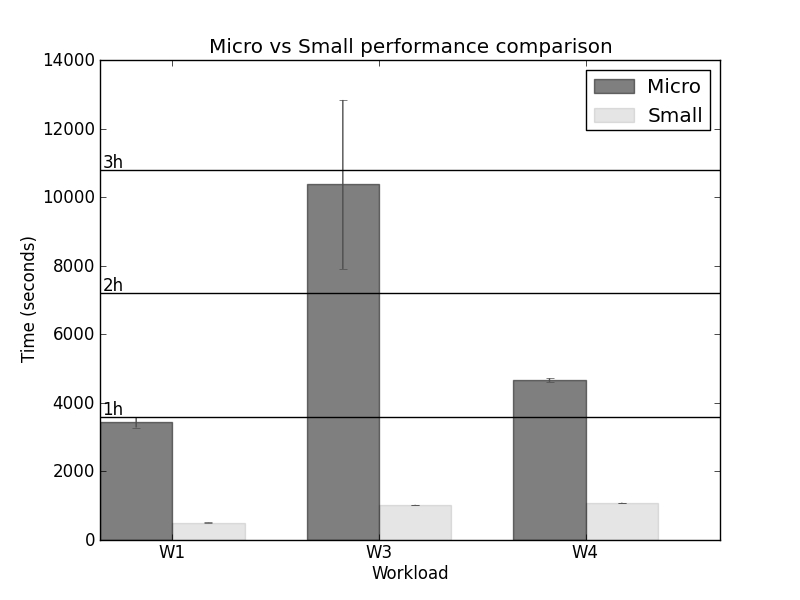
\includegraphics[width=\columnwidth]{chapter_cudswap_figures/micro_vs_small.jpg}
\caption[Comparison of the different workload performance between the Micro instance and the Small instance]{\textbf{Comparison of the different workload performance between the Micro instance and the Small instance.}}
\label{cudswapfigure2}
\end{figure}

Next, we ran the four workloads on the Micro instance and the Small instance,
in which the Micro instance VM incorporates the CUDSwap kernel extension. Figure
\ref{cudswapfigure2} shows the results obtained for different workloads.
The results of the Workload 2 are not shown in the figure for
clarity. While it took only about 8 minutes for Workload 2 to be executed
on the small
instance, it did not finish even after 20 hours in the micro instance.
This huge difference is caused by the fact that Workload 2 is designed
to remove memory locality completely. As a result,
each time the process tries to access a memory location, it is almost always
located
on the swap space, causing the system to swap pages in and out aggressively.

Our first observation is that none of our jobs on Micro instance were
killed, indicating that CUDSwap successfully created new swap space and
prevented calls to OOM killer. Of course, in each case, the execution time
on the Micro instance is considerably larger than the execution time on the
Small instance. Nevertheless, it is important to note that CUDSwap
enables completion of a job despite an incorrect estimation of memory
requirements.

Performance on the Micro instance was slower than the performance on the
Small instance by 6.73X for Workload 1, 10.14X for Workload 3, and 4.32X
for Workload 4. However, since Amazon EC2 works as a pay-as-you-go service,
we should take into account the cost of instances in our evaluation too,
in addition to the performance. From the cost information in Table
\ref{cudswaptable1}, we notice that the execution times of Workloads 1
and 4 are less than two hours, and so, using a Micro instance with CUDSwap
will be cheaper than using a Small instance (\$0.02 versus \$0.06 for
Workload 1, and \$0.04 versus \$0.06 for Workload 4).
For Workload 3, however, there is no benefit of using a Micro instance
with CUDSwap instead of using a Small instance. Most of the time they will
have the same cost (\$0.06), and sometimes the Micro instance may be more
expensive if ends up taking more than 3 hours to complete the job (\$0.08).

So, based on these workloads, we notice that CUDSwap may result in reducing
the cost to a user in some cases, but will result in higher execution times.
However, it is important to note that CUDSwap is designed for situations
where a user makes an incorrect estimation of his/her memory requirements.
In such cases, the user will start his/her job on a Micro instance, incur
the cost of Micro instance, notice that the job has been killed, and then
start the job again on a Small instance and thus incur the cost of Small
instance in addition. In this situation, the cost of running Workload 3
on Micro instance is also cheaper than the cost of running it first
on Micro instance and then later on the Small instance (\$0.06 in the first
case versus \$0.08 in the second case). Furthermore, while considering the
performance in the second case, we should also take into account the time
lost due to first running the job partially on Micro instance and then
setting up a Small instance and restarting the job. This time could be
several minutes or even more depending on when the job on the Micro instance
is killed. So, even in terms of performance, CUDSwap may result in saving
time. Finally, CUDSwap provides a better user experience. Users
(especially non-computer scientists) will typically get annoyed or
frustrated when they see their jobs being killed and losing all the
work after running for some amount time. CUDSwap avoids this situation.

\subsubsection{Small vs Medium Instance}

In order to compare the Small instance versus the Medium instance we have
changed the parameters of our workloads. In this case, for Workloads 1
and 3, we have used a chunk of memory of 2GB. Due to the results obtained
in our previous test, we have not used Workload 2 here, as it will have
very poor performance on the Small instance and we are not going to get
any benefit. For Workload 4, we have used the same subset of 1,000,000
input sequences, but we have used the 99\% representative sequence set
from the GreenGenes database. With these parameters, Workload 4 uses about
2.28 GB of memory. Again, we first ran all three workloads on the Small
instance running standard VM without the CUDSwap kernel extension. In all
three cases, our jobs were killed after a few minutes of execution.

\begin{figure}[htbp]
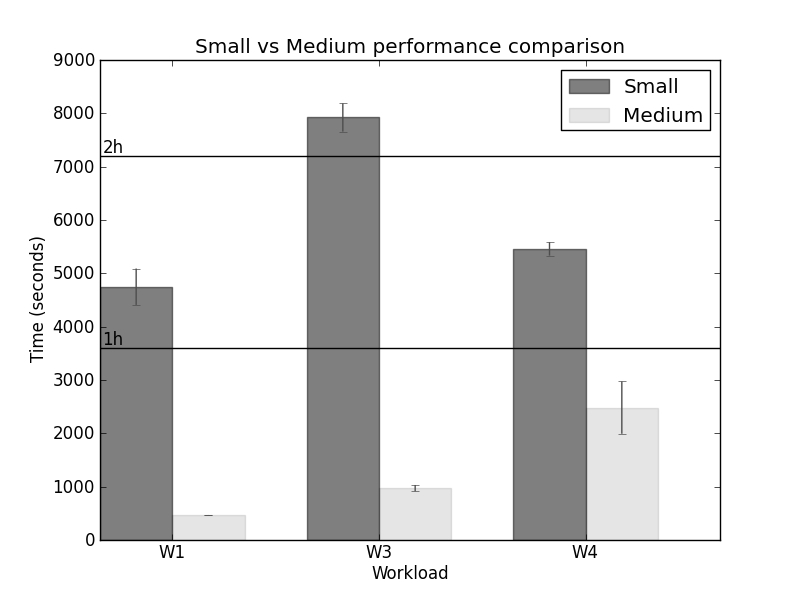
\includegraphics[width=\columnwidth]{chapter_cudswap_figures/small_vs_medium.jpg}
\caption[Comparison of the different workload performance between the Small instance and the Medium instance]{\textbf{Comparison of the different workload performance between the Small instance and the Medium instance.}}
\label{cudswapfigure3}
\end{figure}

Next, we ran the three workloads on the Small instance and the Medium instance,
in which the Small instance VM incorporates the CUDSwap kernel extension.
Figure \ref{cudswapfigure3} shows the results obtained for the
three different workloads. Again, our first observation is that none of
our jobs on Small instance were killed, indicating that CUDSwap successfully
created new swap space and prevented calls to OOM killer. Of course, in each
case, the execution time on the Small instance is considerably larger than
the execution time on the Medium instance.

Performance degradation on the Small instance in comparison to the Medium
instance is 10.01X for Workload 1, 8.14X for Workload 3 and 2.20X for
Workload 4. In terms of cost incrurred in using a Small instance with
CUDSwap versus using a Medium instance, we see that there is no advantage
of using CUDSwap. The cost is same for Workloads 1 and 4 (\$0.12) and
more expensive for workload 3 (\$0.18 for Small instance versus \$0.12 for
Medium instance). However, considering the scenario where a user first starts
his/her job on a Small instance, notices that the job is killed, and then
restarts the job on Medium instance, we see a cost advantage of using
the Small instance with CUDSwap. The cost is \$0.12 for Workloads 1
and 4 running on Small instance with CUDSwap versus \$0.18 or \$0.24 for
the Small/Medium instance scenario outlined above. Similarly, for
Workload 3, the cost is \$0.18 for Small instance and \$0.18, \$0.24 or
\$0.30 for the Small/Medium instance scenario.

In addition, the last two observations we made in Subsection \ref{micro-small}
are relevant here as well. When we take into account the time
lost due to first running the job partially on Small instance and then
setting up a Medium instance and restarting the job, CUDSwap may result in
saving time as well. Finally, CUDSwap provides a better user experience
by preventing calls to OOM killer and ensuring that the user job is
not killed even when the user incorrectly estimates his/her memory requirements.

\subsubsection{Performance Overhead of CUDSwap}

Since CUDSwap is a monitoring module that is always running on the system,
an application incurs the monitoring overhead even if it never needs
additional swap space. Thus, it is important to evaluate the performance
overhead incurred due to CUDSwap usage. Monitoring overhead of CUDSwap
comes from the inception of every {\it do\_brk} and {\it do\_mmap} calls
that the application makes. These calls are made whenever the application
requests new memory.

To estimate this overhead, we ran Workload 1 and Workload 4 on a Medium
instance under two different configurations, on a standard Linux kernel
without CUDSwap kernel extensions and on a Linux Kernel with CUDSwap kernel
extension. For Workload 1, we used 2GB of memory, and for Workload 4,
we used the same configuration as the one we used in our Small versus Medium
experiment. Workloads 2 and 3 have the same memory
allocation (memory request) patterns as Workload 1 and since CUDSwap only
interferes during the allocation process, their overhead will be same as
that in Workload 1.

Figure \ref{cudswapfigure4} shows the results of the
experiment. As we can see in the plot, performance overhead incurred
by CUDSwap is negligible (less than 1\%). This means there is no downside
to using CUDSwap continuously in the system even when the memory
requirements of the jobs have been correctly estimated by the user
and no new swap space is needed.

\begin{figure}[htbp]
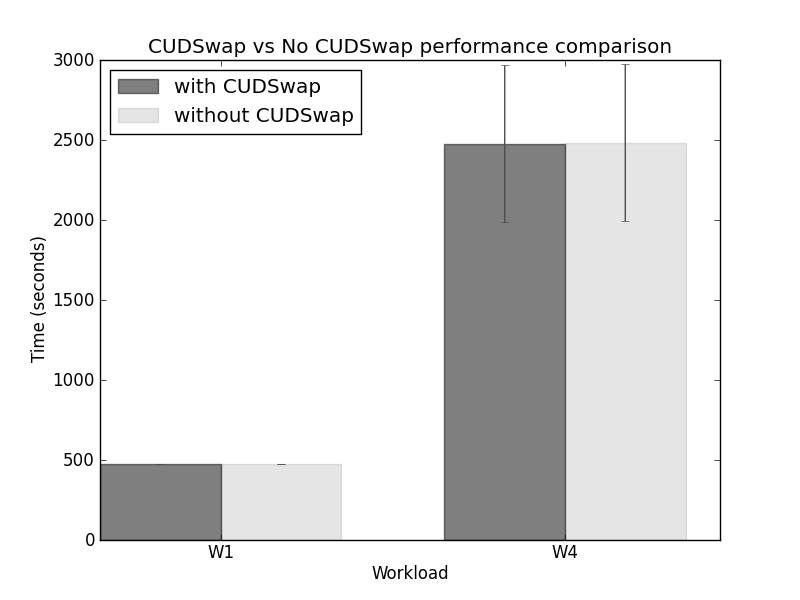
\includegraphics[width=\columnwidth]{chapter_cudswap_figures/with_vs_without.jpg}
\caption[Comparison of Workloads 1 and 4 performance on a Medium instance with and without CUDSwap]{\textbf{Comparison of Workloads 1 and 4 performance on a Medium instance with and without CUDSwap.}}
\label{cudswapfigure4}
\end{figure}

\subsection{Conclusion}\label{sub_cudswap_Conclusion}

We have presented and evaluated CUDSwap, a memory
monitor for guest operating systems that automatically adds virtual memory
to the system creating a swap space when the VM is running out of memory.
Memory is the most expensive resource in a cloud environment and
any memory oversubscription cost is shifted to the end user. Our evaluation
demonstrates that CUDSwap prevents calls to OOM killer when the VM is
short on memory by detecting this situation and adding more swap
space. Furthermore, overhead of CUDSwap is negligible under normal
circumstances when the VM has sufficient memory.

CUDSwap enables completion of a job despite an incorrect estimation of memory
requirements. This is an important functionality because it is
difficult for most cloud users to estimate accurately their application's
memory requirements. In such circumstances, users may either oversubscribe
by renting larger instances than needed, or undersubscribe by renting a
smaller instance than needed and incurring job failure. In both cases, users
end up spending more money. CUDSwap enables users to save money in
situations where users may undersubscribe. In fact, our evaluation shows
that CUDSwap also enables overall time saving for the user in case of
undersubscription, if we consider the entire duration of staring a job
on smaller instance, incurring job failure after some partial execution and
then subscribing a larger instance. So, overall CUDSwap is very useful
in terms of saving both time and money for a user who undersubscribes
due to an incorrect estimation of his/her memory requirements.

While computing with the cloud, multiple evaluation criteria should be taken
into account. Specifically, Cloud computing costs incurred by the user are
as important as the running time of the computing job.
Actual tradeoff should be left to the user. A user may choose to incur
high runtime cost on a lower budget, while another user may choose to incur
low runtime cost on a high budget.
Thus, although applications may be running up to 10X slower due to process
thrashing, the results presented on section \ref{sub_cudswap_Evaluation} show that
a user can save money. Thus, a user may choose to undersubscribe his/her
instance in favor of reducing the costs of using the cloud.

There is another subtle advantage of using CUDSwap in the form of better
user experience. In a scenario where a user encounters a failure and restarts
his/her job on a larger instance, he/she may get annoyed or frustrated
feeling that he/she has wasted time and money. CUDSwap avoids this
scenario.

In general, CUDSwap is useful only when there is difficulty in estimating the
memory requirements of a job. If a user can accurately predict his/her
memory requirements, he/she should certainly subscribe the instance
that provides sufficient memory for job completion, and not undersubscribe
and depend on CUDSwap.

CUDSwap is being used
by several graduate students in the BioFrontiers Institute at our university.
Jose Antonio Navas-Molina is a graduate student of the
BioFrontiers Institute and started working on CUDSwap after encountering
the memory undersubscription problem.
Our current implementation of CUDSwap is quite stable.
Nevertheless, there are some
additional future directions that we are addressing. At present,
CUDSwap intercepts {\it do\_brk} and {\it do\_mmap} systems calls.
Another way of consuming memory in the system is by a forking new
process, which creates a new process and a new chunk of memory needs to
be allocated for the new process. This situation can also be detected using
the Jprobes system and we plan to incorporate it in CUDSwap in the future.

Another area that we plan to investigate is the utility of CUDSwap
for applications that have widely varying memory requirements with
very short periods of peak requirements. In the absence of CUDSwap, a user
will have to subscribe a larger instance to satisfy these peak requirements.
With CUDSwap, it may be more optimal to subscribe a smaller instance, since
the time in actual swapping will be short.

\subsection{Acknowledgments}

Jose Antonio Navas-Molina is supported by the Balsells fellowship.
